\chapter{Design}
\label{ch:design}

為了自動化探索可能的選項、選項參數，本研究提出一種全新的多參數模糊測試架構。首先結合靜態分析、動態分析，找出目標程式中可用的選項並合理地組合。接著利用污染源推論，針各個選項的選項參數進行分析，根據推論的結果變異選項參數。同時改良模糊測試工具的 forkserver，使其能夠在不關閉重起的情況下，替換目標程式使用的參數。這個架構能夠根據執行階段提供的回饋，動態地調整選項的組合、選項參數的值，因此稱為選項感知模糊測試（Option-Aware Fuzzing）。我們設計並實做了對應的開源原型：KOFTA。

\section{選項分析}

要尋找目標程式可接受的選項相對簡單，只需要分析相關常用於解析參數的函式，例如 \texttt{strcmp()}、 \texttt{getopt()}、 \texttt{getopt\_long()} 即可。也因為選項通常是固定不變的、在目標程式原始碼中就已經確定，因此編譯階段的靜態分析適用於尋找可用的選項。

一個專案中可能包含多個可執行檔，例如 GNU Binutils 專案中包含了多個用於分析處理二進制檔案的工具：objdump、ar、ranlib 等等。然而專案不一定會提供個別編譯可執行檔的步驟方法，如 Binutils 就無法單獨編譯 objdump（未紀錄於相關文件中），必須連同其他工具一起編譯。此時靜態分析的結果將無法確定特定選項應該屬於哪一個可執行檔。因此需要透過蒐集執行階段的回饋，動態分析正確可用的選項組合。

\subsection{靜態分析}
\label{subsec:optana-static}

在 C 標準函式庫中有提供 \texttt{getopt()} 用於分析短選項：

\begin{lstlisting}[numbers=none]
int getopt(int argc, char * const argv[],
           const char *optstring);
\end{lstlisting}

其中 \texttt{optstring} 字串會描述有哪些可用的短選項，是我們分析的重點：

\begin{lstlisting}[numbers=none]
"abc:d::"
\end{lstlisting}

這個 \texttt{optstring} 中描述了 \texttt{a}、\texttt{b}、\texttt{c}、\texttt{d} 四個短選項，選項字元後可接零至二個「 \texttt{:} 」代表該選項的「選項參數必要性」。零個「\texttt{:}」代表該選項單獨使用，「無」選項參數；一個「\texttt{:}」代表該選項之選項參數為「必要」，不可單獨使用；兩個「\texttt{:}」則代表選項參數「非必要」，選項可以單獨使用。

對於長選項的解析，GNU 標準的擴充（extension）提供了：

\begin{lstlisting}[numbers=none]
int getopt_long(int argc, char * const argv[],
                const char *optstring,
                const struct option *longopts,
                int *longindex);
\end{lstlisting}

函式的前三個參數與 \texttt{getopt()} 相同，其中的 \texttt{optstring} 可以用於分析短選項；不同的是，第四個參數描述了可用的長選項，參數 \texttt{longopts} 是一個結構陣列（structure array），陣列中每個項目都是一個 struct option 結構：

\newpage

\begin{lstlisting}[numbers=none]
struct option {
    const char *name;
    int         has_arg;
    int        *flag;
    int         val;
};
\end{lstlisting}

結構中的第一個成員 \texttt{name} 是長選項的名稱；第二個成員 \texttt{has\_arg} 代表該選項的選項參數必要性，同樣分為「無」、「必要」、「非必要」選項參數；第四個成員是一個整數，若該整數位於可視字元的 ASCII 區間內，則經常代表該長選項對應的短選項。除此之外，也有一些程式單純使用字串匹配的方式實現命令列參數解析（如 Listing \ref{lst:xmllint-argparse}）。因此分析 \texttt{strcmp()} 的字串參數是否以「\texttt{-}」開頭，也有助於尋找可用的選項。

在編譯階段，透過分析 \texttt{optstring}、\texttt{longopts}、\texttt{strcmp()} 的字串參數，便能夠從原始碼中提取可用的選項，以及該選項的選項參數必要性。在這個階段，透過 \texttt{strcmp()} 找到的選項暫時無法確定其選項參數必要性，因此將先標記為「非必要」。

\subsection{選項組合}

目標程式在編譯時，可能需要連同專案中其他的可執行檔一起編譯，然而這些可執行檔間往往會共用部份的原始碼檔案。例如 GNU Binutils 中的 ar 和 ranlib 在編譯時都會需要 ar.c 這份原始碼，因此靜態分析時從 ar.c 中提取的選項，將無法確定應該屬於 ar 或是 ranlib。為了解決這個問題，在分析 \texttt{strcmp()}、 \texttt{getopt()}、 \texttt{getopt\_long()} 等等關鍵函式的同時，會生成一個隨機的識別碼，並在該關鍵函式呼叫處（call site）前插樁，用於執行時回報該識別碼。

如同範例（Listing \ref{lst:optana-instrument}）所示，在分析 \texttt{getopt()} 的同時會產生一個隨機的識別碼：\texttt{23927}，並將該識別碼作為函式 \texttt{\_\_kofta\_optana()} 的參數，插樁在 \texttt{getopt()} 之前呼叫。實際執行目標程式時 \texttt{\_\_kofta\_optana()} 會紀錄所有呼叫過的識別碼，紀錄的識別碼會作為執行階段的回饋。KOFTA 會根據動態分析蒐集的識別碼搜尋靜態分析中對應的可用選項；在這個範例中，目標程式執行後 KOFTA 會根據識別碼 \texttt{23927} 找到有 \texttt{-n} 及 \texttt{-t} 兩個可用選項，後續就可以組合這些選項產生下一次的測試。

這項設計同時帶來了另一個好處：可以提高選項組合合法的機率。考慮一個巢狀的參數解析（Listing \ref{lst:optana-nested}），只有當第一個參數是 \texttt{--foo} 時，第二個參數 \texttt{--bar} 作為選項才有意義。設想在第一次不帶任何參數的測試執行後，KOFTA 會根據執行階段回饋的識別碼 \texttt{62376} 產生帶有 \texttt{--foo} 的下一組測試；帶有 \texttt{--foo} 參數的測試在執行階段將回饋兩個識別碼：\texttt{62376} 與 \texttt{11514}，因此下一組衍生的測試參數可能是 \texttt{--foo --foo} 或是 \texttt{--foo --bar}，後者可以順利進入巢狀結構的最內層，只有前者將是一次冗餘的測試。相較於過去研究中使用的參數組態檔，其無法描述選項之間的相依性，即使在沒有 \texttt{--foo} 選項的情況下，仍然可能產生很多包含 \texttt{--bar} 選項的測試，這些測試都將是無效而且浪費時間的；這個設計將提昇選項組合的測試效率。

\vfill

\begin{lstlisting}[caption=選項動態分析插樁範例, label=lst:optana-instrument]
int main(int argc, char** argv) {

    __kofta_optana(23927);
    while ((opt = getopt(argc, argv, "nt:")) != -1)
    {
        // ...
    }

}
\end{lstlisting}

\begin{lstlisting}[caption=巢狀參數解析範例, label=lst:optana-nested]
int main(int argc, char** argv) {

    __kofta_optana(62376);
    if (!strcmp(argv[0], "--foo"))
    {
        __kofta_optana(11514);
        if (!strcmp(argv[1], "--bar"))
        {
            // ...
        }
    }

}
\end{lstlisting}

\subsection{選項參數必要性評估}

本研究與過去相關研究最大的不同在於，透過污染源分析的方法探索選項參數廣闊的輸入空間，因此確認一個選項是否能夠帶有選項參數至關重要；選項參數必要性分為三類：無、必要、非必要。非必要的選項參數通常代表其存在預設值（default value），當該選項不帶選項參數、單獨使用時，選項參數的預設值便會是實際使用的值。然而不帶選項參數就無法使用污染源分析、只使用預設值便會失去探索其他路徑的機會，這對於覆蓋率導向的模糊測試而言是不利的。因此 KOFTA 對於「非必要」的選項參數會更傾向於使其「必要」，也就是為該選項帶入選項參數，探索更多可能的執行路徑。

然而在靜態分析階段中，由於無法確定藉由分析 \texttt{strcmp()} 所提取的選項的選項參數必要性，因此會先將其標記為「非必要」（\S \ref{subsec:optana-static}）；即使是透過分析 \texttt{optstring} 或 \texttt{longopts} 找到的選項，標記為「非必要」選項參數的選項在解析時也可能實際上是「無」選項參數。如同範例（Listing \ref{lst:optional-arg}）所示，靜態分析後可以知道「 \texttt{--disassemble} 」的選項參數必要性為「非必要」（\texttt{optional\_argument}），然而 objdump 實際在解析時卻將其視為一個「無」選項參數的選項（Line 13-17）。由此可見，貿然地將選項參數必要性中「非必要」皆視為「必要」是不可行的，必須有一個蒐集執行階段回饋以評估選項參數必要性的方法。

\begin{lstlisting}[caption=\texttt{objdump} 非必要選項參數範例, label=lst:optional-arg]
static struct option longopts[]=
{
  {"disassemble", optional_argument, NULL, 'd'},
};

int main (int argc, char **argv)
{
  while ((c = getopt_long (argc, argv, optstring,
                           longopts, NULL)) != EOF)
  {
    switch (c)
    {
    case 'd':
      disassemble = true;
      disassemble_all = true;
      seenflag = true;
      break;
    }
  }
}
\end{lstlisting}

\begin{lstlisting}[language=sh, caption=程式退出碼範例一, label=lst:exit-code-1]
$ objdump -d &> /dev/null 
$ echo $?                                
0
$ objdump -d xyz &> /dev/null
$ echo $?                                    
1
\end{lstlisting}

要觀察使用的選項、選項參數是否合法，一個簡單的方法是檢查目標程式的退出碼（exit code），慣例上通常以退出碼「 \texttt{0} 」表示程式正常執行、退出碼「非 \texttt{0} 」表示程式執行期間出現錯誤（Listing \ref{lst:exit-code-1}）。退出碼將作為執行階段的回饋交由 KOFTA 進行評估。針對「非必要」的選項參數，評估其選項參數必要性的方法主要分為三個階段。

第一階段會將「\texttt{0}」作為該選項的選項參數填充值進行測試，例如要測試的選項為「\texttt{-d}」便會產生「\texttt{-d 0}」。當測試執行後會檢查目標程式的退出碼，如果退出碼為「\texttt{0}」代表目標程式順利執行，便會將該選項的選項參數必要性重新標記為「必要」並結束評估；然而當退出碼為「非 \texttt{0}」時，並不一定代表該選項不能帶有選項參數，有可能是因為帶入的填充值「\texttt{0}」本身不是一個合法的選項參數。如同範例（Listing \ref{lst:exit-code-2}）所示，選項「\texttt{-m}」本身可以帶有選項參數，執行「\texttt{-m i386}」後的退出碼為 \texttt{0}；而「\texttt{xyz}」並非選項「\texttt{-m}」的合法選項參數，因此執行「\texttt{-m xyz}」後的退出碼不為 \texttt{0}。要評估這類選項的選項參數必要性需要進入下一個階段。

\begin{lstlisting}[language=sh, caption=程式退出碼範例二, label=lst:exit-code-2]
$ objdump -d -m i386 &> /dev/null
$ echo $?                                        
0
$ objdump -d -m xyz &> /dev/null
$ echo $?                                        
1
\end{lstlisting}

第二階段會針對仍無法確定選項參數必要性的選項進行污染源推論，污染源推論的結果是一系列的「提示」，每個提示都有可能是該選項合法的選項參數之一（\S \ref{sec:args-explo}）。接著將提示逐一替換為選項參數的值進行測試。例如，對「\texttt{-m 0}」進行污染源推論後得到三個提示：\texttt{abc}、\texttt{i386}、\texttt{xyz}，便會逐一測試 \texttt{-m abc}、\texttt{-m i386} 與 \texttt{-m xyz}。一旦發現任何可用的選項參數（退出碼為 \texttt{0}），便會將該選項的選項參數必要性重新標記為「必要」並結束評估；反之需要進入第三個階段。

在最後一個階段中，會將選項不帶選項參數單獨進行測試，如果發現退出碼為 \texttt{0}，便會將該選項的選項參數必要性重新標記為「無」；反之則代表所有階段中的測試皆產生退出碼為非 \texttt{0} 的結果，這可能是因為與其他選項的組合不合法、或是與輸入檔的組合不合法，導致無法確定該選項的選項參數必要性，KOFTA 將維持其參數必要性不變、仍標記為「非必要」。

\section{選項參數探索}
\label{sec:args-explo}

相比於選項，選項參數缺乏明顯的特徵，而且通常有更多的可能性，難以使用靜態分析直接從原始碼中提取。因此本研究使用污染源推論的方法，在執行階段找出選項參數可能的值作為「提示」回饋；同時探索提示與選項之間的關聯性，將選項與對應的選項參數進行合理的組合。

過去污染源推論與模糊測試的研究中，為了講求分析的準確性，會捨棄所有不確定的結果。但這對於選項參數的探索來說是不利的，因此本研究提出一種基於雜湊的折衷方法，犧牲部份的推論準確性、提昇選項參數探索的能力。

\subsection{污染源推論}

使用不同的選項參數測試是為了提高測試覆蓋率，不同的選項參數有機會走訪不同的分支進而產生新的執行路徑。因此觀測選項參數如何影響特定分支條件成為了增加覆蓋率的關鍵。污染源推論用於分析資料流，推論外部的輸入是否能夠影響程式執行時內部的記憶體。如果將選項參數設為污染源、分支條件設為污染終點，便能推論前者是否能影響後者。

所有的選項參數可以分為兩大類：字串與數值。與字串相關的分支條件經常使用 \texttt{strcmp()} 來判斷該選項參數是否合法；數值相關的選項參數也會經由 \texttt{if-else} 的條件檢查是否在合法的範圍。因此  \texttt{strcmp()} 的參數、 \texttt{if-else} 條件的運算元都可以作為選項參數的「提示」考慮。例如在範例（Listing \ref{lst:argparse-example}）中，與選項 \texttt{--foo} 相關的提示是 \texttt{if-else} 條件中的運算元「\texttt{100}」；與選項 \texttt{--bar} 相關的提示是 \texttt{strcmp()} 的參數「\texttt{xyz}」。根據這些提示 KOFTA 會產生 \texttt{--foo 99}、\texttt{--foo 100}、\texttt{--foo 101} 及 \texttt{--bar xyz} 等等一系列的測試，嘗試通過這些分支條件。

\begin{lstlisting}[caption=選項參數解析範例, label=lst:argparse-example]
  if (!strcmp(argv[i], "--foo"))
  {
    if (atoi(argv[i+1]) < 100)
    {
      // ...
    }
  }
  if (!strcmp(argv[i], "--bar"))
  {
    if (!strcmp(argv[i+1], "xyz"))
    {
      // ...
    }
  }
\end{lstlisting}

要完成污染源推論首先需要在編譯階段對各個污染終點插樁，接著透過這些插樁在執行階段蒐集執行路徑上污染終點的狀態，每個污染終點會根據狀態計算雜湊、紀錄為一個節點，多個節點串連形成一個能夠代表該執行路徑的鏈結串列（linked list）；若比較兩個鏈結串列，便可以知道兩個執行路徑在何時發生分歧。

我們感興趣的污染終點除了 \texttt{strcmp()} 的字串參數、\texttt{if-else} 比較條件的運算元以外，還有 \texttt{switch-case} 的運算元及其各個目標（case）的值。如同範例（Listing \ref{lst:tntsnk-example}）所示，在 \texttt{strcmp()} 之前會有 \texttt{\_\_kofta\_trace\_str()} 插樁，兩者參數相同；在 \texttt{if-else} 比較條件之前會有 \texttt{\_\_kofta\_trace\_cmp()} 插樁，並將比較條件的左、右運算元作為參數；在 \texttt{switch-case} 之前會有 \texttt{\_\_kofta\_trace\_swt()} 插樁，第一個參數是目標的數量、第二個參數是包含所有目標的陣列、第三個參數是比較的運算子。這三個插樁的函式會根據傳入的參數計算雜湊值，形成一個新的節點至目前的鏈結串列中。

考慮以下目標程式（Listing \ref{lst:tntana-exec-example1}）中，要對選項「\texttt{--kofta}」的選項參數進行污染源推論，至少需要執行目標程式兩次。假設第一次以「\texttt{--kofta foo}」執行，至少會在鏈結串列中產生四個節點：strcmp（Line 3）、ifcmp（Line 3）、ifcmp（Line 7）、ifcmp（Line 10），代表本次測試的執行路徑（Figure \ref{fig:tntana-exec-example1}）。接著第二次測試中，我們將選項「\texttt{--kofta}」的選項參數改變後以「\texttt{--kofta xyz}」執行，在這次測試的執行路徑中同樣會產生四個鏈結串列的節點；不同的是，從第三個節點開始與第一次執行的結果不同（Figure \ref{fig:tntana-exec-example2} 中靠左紅圈處）。因此我們可以推論：選項「\texttt{--kofta}」的選項參數「污染」了該節點的比較條件。而被污染節點上的運算子「\texttt{a}」將作為「提示」回饋，於是 KOFTA 可以根據提示產生「\texttt{--kofta a}」的測試、產生新的測試覆蓋率。

\vfill

\begin{figure}
     \centering
     \begin{subfigure}[]{\textwidth}
         \centering
         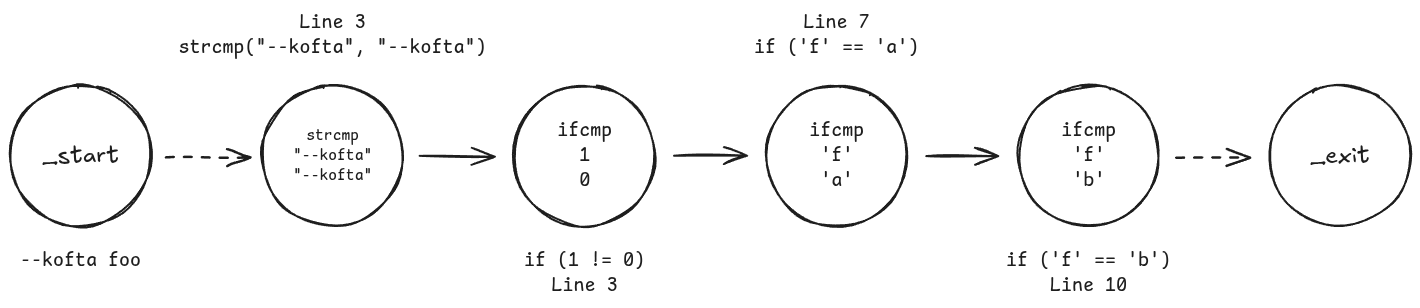
\includegraphics[width=\textwidth]{img/tntana-exec-example1.png}
         \caption{測試 \texttt{--kofta foo} 產生的執行路徑}
         \label{fig:tntana-exec-example1}
     \end{subfigure}
     \begin{subfigure}[]{\textwidth}
         \centering
         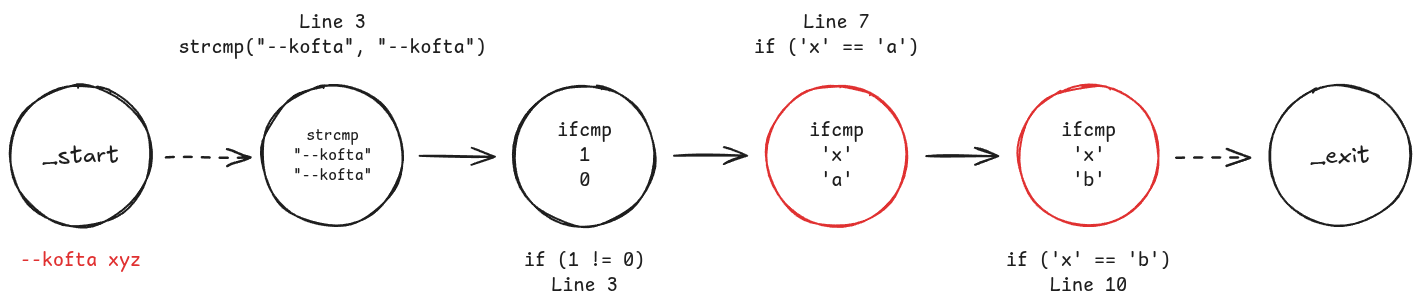
\includegraphics[width=\textwidth]{img/tntana-exec-example2.png}
         \caption{測試 \texttt{--kofta xyz} 產生的執行路徑}
         \label{fig:tntana-exec-example2}
     \end{subfigure}
        \caption{污染源分析鏈結串列範例}
        \label{fig:tntana-lnklst-example}
\end{figure}

\begin{lstlisting}[caption=污染源推論執行範例一, label=lst:tntana-exec-example1]
int mode = MODE_NONE;
if (!strcmp(argv[i], "--kofta")) {
  char arg = argv[i++][0];
  if (arg == 'a') {
    mode = MODE_A;
  }
  else if (arg == 'b') {
    mode = MODE_B;
  }
}
\end{lstlisting}

\begin{lstlisting}[caption=污染終點插樁範例, label=lst:tntsnk-example]
  __kofta_trace_str(argv[i], "i386");
  __kofta_trace_cmp(!strcmp(argv[i], "i386"), 0);
  if (!strcmp(argv[i], "i386"))
  {
    // ...
  }
  __kofta_trace_cmp(atoi(argv[i]), 100);
  if (atoi(argv[i]) < 100)
  {
    // ...
  }
  __kofta_trace_swt(2, {'x', 'y'}, argv[i][0]);
  switch (argv[i][0])
  {
    case 'x':
      // ...
      break;
    case 'y':
      // ...
      break;
  }
\end{lstlisting}

\subsection{污染終點特徵值}
\label{subsec:tntana-chara}

在前面的例子（Figure \ref{fig:tntana-lnklst-example}）中，除了第三個節點以外，實際上第四個節點（Figure \ref{fig:tntana-exec-example2} 中靠右紅圈處）也是被污染的污染終點。然而過去將污染源推論與模糊測試結合的研究中，認為一旦發現第一個被污染的污染終點，後續的污染終點將沒有參考價值。因為當比較條件的運算元改變，代表後續的執行路徑很有可能也發生改變，此時再去比較兩個鏈結串列的節點已經沒有意義。這樣的作法提高了污染源推論的準確性，但同時也捨棄了所有其他可能被污染的污染終點；導致 KOFTA 無法在本例（Listing \ref{lst:tntana-exec-example1}）中推論出「\texttt{--kofta b}」這個選項參數的組合，因此需要一種方法判斷這種由 \texttt{if-else} 組成的「污染終點群組」，若群組中比較的對象相同（Line 7,10 皆比較 \texttt{arg}）則應將群組中比較條件的運算子（Line 7 的 \texttt{a} 與 Line 10 的 \texttt{b}）皆作為提示回饋。

為了判斷污染群組中比較的對象是否相同，會根據該節點的「比較對象」與「污染終點類型（\texttt{strcmp()}、\texttt{if-else} 或 \texttt{switch-case}） 」計算一個雜湊值、稱為該污染終點的「特徵值」。換句話說，當兩個相同類型的污染終點的比較對象也相同時，兩個節點將會有相同的特徵值。在發現第一個被污染的污染終點時紀錄其特徵值，與後續相鄰的節點比較，如果兩兩特徵值相同，代表它們可能屬於同一個污染終點群組、且有相同的比較對象，應將比較條件的運算元皆作為提示回饋（Figure \ref{fig:tntana-group-example}）；這個比較會持續到發現第一個特徵值不同的節點為止。

\vfill

\begin{figure}[hb]
    \centering
    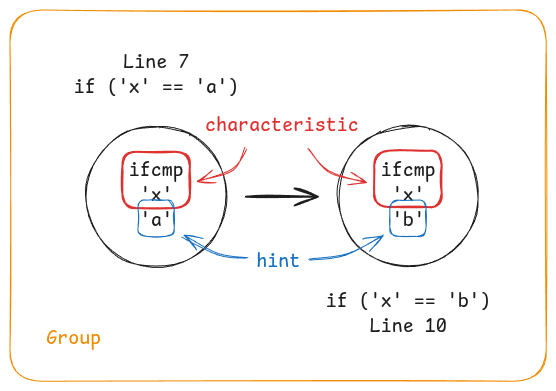
\includegraphics[width=0.5\textwidth]{img/tntana-group-example.png}
    \caption{污染終點群組、特徵值、提示範例}
    \label{fig:tntana-group-example}
\end{figure}

\begin{figure}[ht]
    \centering
    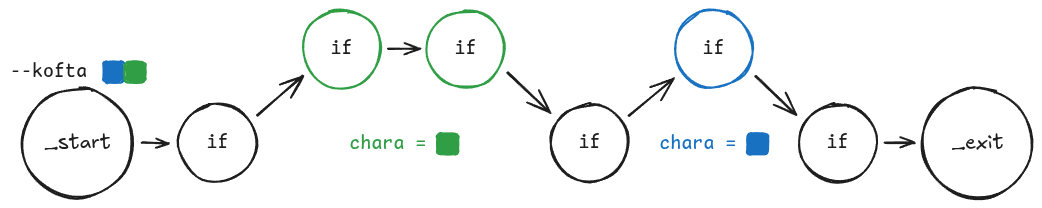
\includegraphics[width=\textwidth]{img/tntana-dscgrp-example.png}
    \caption{非連續污染終點群組範例}
    \label{fig:tntana-dscgrp-example}
\end{figure}

\subsection{非連續污染終點群組}

在污染源推論中加上特徵值作為參考，雖然可能降低推論的準確性，但能提供更多潛在污染終點的提示，這對於選項參數的探索是十分有利的；然而只考慮一個污染終點群組內部的節點仍然是不夠的。試想以下的鏈結串列（Figure \ref{fig:tntana-dscgrp-example}）中，綠色圓圈與藍色圓圈的節點皆是被選項「\texttt{--kofta}」的選項參數污染的污染終點。其中兩個相鄰的綠色圓圈有相同的特徵值，組成了污染終點群組並且可以被 \S \ref{subsec:tntana-chara} 中的方法識別；然而藍色圓圈不僅沒有與綠色圓圈的污染終點群組相連，其特徵值也與綠色節點的不同。為了識別藍色圓圈的污染終點，還需要額外的判斷。

當污染終點群組結束後，可以比較下一個節點是否與原先鏈結串列中對應位置的節點相同。如果發現節點相同，可以視為前面被污染的節點的比較條件運算子雖然改變，但並因此未走訪不同的分支；既然仍在相同執行路徑上，便能夠繼續比較兩個鏈結串列中的節點是否相同。此時發現藍色圓圈的節點產生分歧，便將它視為一個新的污染終點群組，紀錄其特徵值與後續的節點做比較。

\section{多參數 forkserver}

除了評估選項參數必要性時需要使用污染源推論，探索選項參數的方法也是建立於污染源推論之上。而污染源推論的原理是觀察一個選項帶有不同的選項參數時，執行路徑上的污染終點的狀態是否發生改變。由此可見，目標程式的命列列參數需要經常改變；若是每次改變都需要暫時關閉 forserver，使用 exec 系統呼叫的額外成本將會相當可觀。因此需要改良 AFL 的 forserver，使其在不關閉的情況下也能夠替換目標程式的命令列參數。

\subsection{forkserver 原理}

forkserver 的運作原理是在目標程式中增加了「建構子（constructor）」函式的程式碼片段。如圖（Figure \ref{fig:afl-forkserver}）所示，程式在進入 \texttt{main()} 之前，還會呼叫許多其他函式進行初始化，其中就包括可以由程式自定義的一系列建構子函式；而 forkserver 正是其中之一。forkserver 在使用 \texttt{fork} 呼叫後，子程序會從 \texttt{forkserver} 返回，繼續執行剩餘的建構子函式，最終進入 \texttt{main()} 執行；父程序則會藉由迴圈留在 \texttt{forkserver} 中，等待下一次的 \texttt{fork} 呼叫。

\begin{figure}[hb]
    \centering
    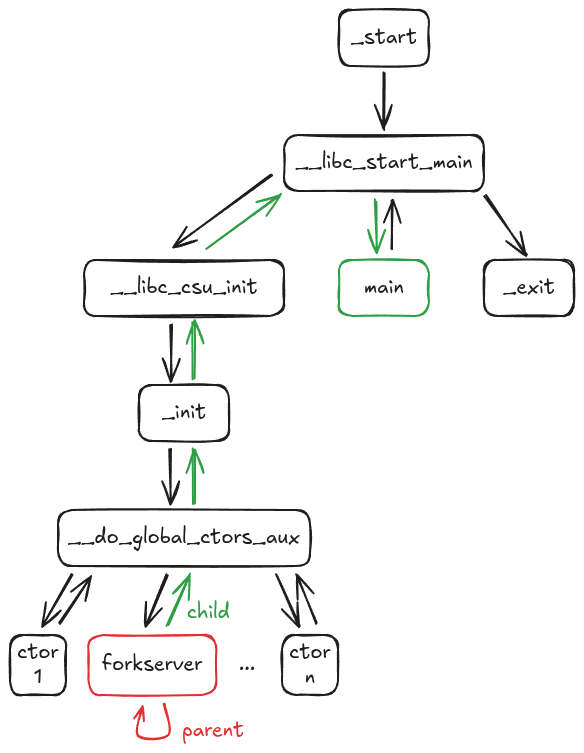
\includegraphics[width=0.6\textwidth]{img/forkserver.png}
    \caption{AFL forkserver}
    \label{fig:afl-forkserver}
\end{figure}

\subsection{命令列參數指標}
\label{subsec:cmdln-argptr}

從流程圖（Figure \ref{fig:afl-forkserver}）中不難發現，\texttt{main()} 由 \texttt{\_\_libc\_start\_main()} 呼叫，因此傳入的參數「\texttt{int argc}」與「\texttt{char *argv[]}」應該也位於其記憶體堆疊（stack）上。又因為從 \texttt{\_\_libc\_start\_main()} 至 forkserver 的路徑單純，對於大部分一般的程式而言，這條執行路徑上產生的記憶體佈局（memory layout）應該皆相同；換言之，從 forkserver 的堆疊至位於 \texttt{\_\_libc\_start\_main()} 堆疊上的「\texttt{argc}」與「\texttt{argv}」的記憶體位置偏移量（offset）應該是一個固定值（Figure \ref{fig:fsrv-memlyt}）。即使這個值可能因為電腦環境不同而發生改變，但是對於本研究固定的實驗環境來說，紀錄並使用該偏移量找到 \texttt{argc} 與 \texttt{argv} 仍然很有幫助。因為知道兩者的位置便可以在使用 fork 呼叫前，修改即將傳入 \texttt{main()} 的命令列參數，實現支援多參數的 forkserver。

\vfill

\begin{figure}[hb]
    \centering
    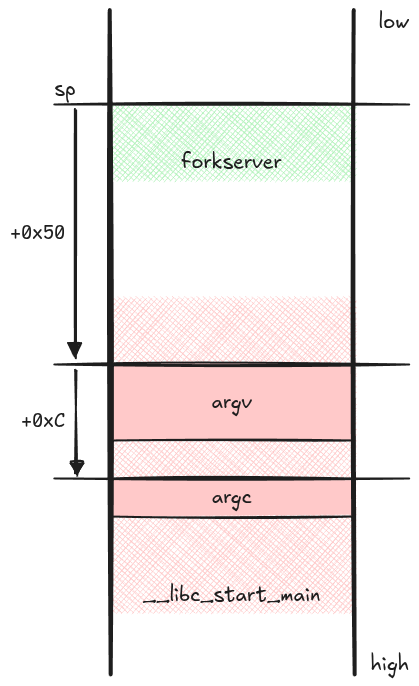
\includegraphics[width=0.45\textwidth]{img/fsrv-memlyt.png}
    \caption{forkserver 記憶體佈局}
    \label{fig:fsrv-memlyt}
\end{figure}